
\documentclass[14pt]{beamer}
\usetheme{Singapore}

% CMU sans serif font.
\usepackage[T1]{fontenc}
\renewcommand*\familydefault{\sfdefault}

% Wrap Figures (\minipage)
\usepackage{graphicx}

% APA 6 citation and bibliography style % Note: Must be loaded after hyperref
\usepackage{apacite} 


%% Math
%\usepackage{amsfonts}
%\usepackage{amsmath}
%
%% Margins
%\usepackage[top=2.4cm,bottom=2.4cm,outer=2.4cm,inner=4.2cm]{geometry}
%
%% Hyperlinks
%\usepackage{hyperref}
%\hypersetup{
%    colorlinks=true,       	% false: boxed links; true: colored links
%    linkcolor=black,          	% color of internal links (change box color with linkbordercolor)
%    citecolor=black,        	% color of links to bibliography
%    filecolor=blue,      		% color of file links
%    urlcolor=blue           	% color of external links
%}
%
%% Abbreviations (Acronyms)
%\usepackage[acronym]{glossaries}
%\makeglossaries
%\newacronym{pisa}{PISA}{Programme for International Student Assessment}
%\newacronym{oecd}{OECD}{Organisation for Economic Co-operation and Development}
%\newacronym{stem}{STEM}{Science, Technology, Engineering and Mathematics}
%\newacronym{fmri}{fMRI}{functional magnetic resonance imaging}
%\newacronym{naplan}{NAPLAN}{National Assessment Program --- Literacy and Numeracy}
%
%\newacronym{ac}{AC}{Australian Curriculum}
%\newacronym{sace}{SACE}{South Australian Certificate of Education}
%\newacronym{amsi}{AMSI}{Australian Mathematical Sciences Institute}
%
%\newacronym{uofa}{UofA}{University of Adelaide}
%\newacronym{ecms}{ECMS}{Faculty of Engineering, Computer and Mathematical Sciences}
%\newacronym{mlc}{MLC}{Maths Learning Centre}
%
%
%% Date by Month for Title Page
%\usepackage{datetime}
%\newdateformat{monthyeardate}{%
%  \monthname[\THEMONTH], \THEYEAR}
%
%% Intentionally Blank Page
%\newcommand*{\intentionallyblankpage}{
%  \vspace*{\fill}
%  {\centering \textit{This page intentionally left blank.} \par}
%  \vspace{\fill}}
%\makeatletter
%\renewcommand*{\cleardoublepage}{\clearpage\if@twoside \ifodd\c@page\else
%  \intentionallyblankpage
%  % \thispagestyle{empty}
%  \newpage
%  \if@twocolumn\hbox{}\newpage\fi\fi\fi}
%\makeatother
%
%% Table of Contents
%%\usepackage[nottoc]{tocbibind}
%\setcounter{tocdepth}{1}
%
%% Section and Figure Numbering
%%\renewcommand\thesection{\arabic{section}}
%%\usepackage{chngcntr}
%%\counterwithout{figure}{chapter}
%%\counterwithout{table}{chapter}
%
%% Referencing Commands
%\newcommand{\refchap}[1]{\hyperref[chap:#1]{Chapter~\ref{chap:#1}}}
%\newcommand{\refsec}[1]{\hyperref[sec:#1]{Section~\ref{sec:#1}}}
%\newcommand{\reffig}[1]{\hyperref[fig:#1]{Figure~\ref{fig:#1}}}
%\newcommand{\reftab}[1]{\hyperref[tab:#1]{Table~\ref{tab:#1}}}
%\newcommand{\refapp}[1]{\hyperref[app:#1]{Appendix~\ref{app:#1}}}


\title{Mathematics Bridging: \\ Aligning MathsTrack to the National Curriculum}
\author{Lyron Winderbaum}
\institute{University of Adelaide}
\date{\today}
\logo{
\includegraphics[scale=0.45]{../files/UoA_logo_col_horiz.png}}

\begin{document}

\begin{frame}
\titlepage
\end{frame}

\begin{frame}
\frametitle{Outline}
\tableofcontents
\end{frame}

\section{Introduction}

\subsection{About Me}
\begin{frame}
\frametitle{About Me}
\begin{minipage}[0.4\textheight]{\textwidth}
\begin{columns}[T]
\begin{column}{0.6\textwidth}
\begin{itemize}
	\item Lyron Winderbaum
	\item Ph.D. in Mathematics
	\item Teaching at UofA since 2010.
\end{itemize}
\end{column}
\begin{column}{0.4\textwidth}
	
\includegraphics[scale=0.1]{../../photos/portrait.jpg}
\end{column}
\end{columns}
\end{minipage}
\end{frame}



\subsection{The What and Why of my Research}

\begin{frame}
\frametitle{My Research Question}
\begin{quote}
	How can MathsTrack be improved?
\end{quote}
\end{frame}

\begin{frame}
\frametitle{What is MathsTrack?}
MathsTrack is a mathematics bridging course offered through the Maths Learning Centre (MLC) at the University of Adelaide (UofA).
% Acknowledge MLC, David, and Nick. 
% Frame research question as me giving back for their inspiration.
\end{frame}

\begin{frame}
\frametitle{Mathematics Bridging}
Mathematics bridging courses attempt to catch students that would otherwise ``fall through the gaps'' in our education system, providing them with a path towards a tertiary mathematics education that might otherwise be unavailable to them.

They serve a crucial stop-gap role in our education system and our society more broadly.
\end{frame}

\begin{frame}
\frametitle{The Mathematics Problem}
Partiticipation in mathematics education has been steadily declining for over three decades.

In the meantime, the Australian and international industries and economies have been becoming steadily more dependant on a mathematically educated workforce.
\end{frame}

\begin{frame}
\frametitle{Equity}
The ``Mathematics Problem'' has two key consequences:
\begin{itemize}
	\item Struggling economies due to reduces supply of capable workforce.
	\item Increased disadvantage in the job market for people without access to a mathematics education.
\end{itemize}
%This second point highlights how mathematics education can create social mobility.
\end{frame}

\begin{frame}
\frametitle{Motivation}
Mathematics bridging is serving an increasingly important role in our education systems worldwide and is getting increased attention due to it's importance to industry and impact on economies, but also it also serves a critically important role in our culture by offering the potential for social mobility.
\end{frame}

\section{My Research}

\begin{frame}
\frametitle{Introduction}
I conducted two parallel avenues of research:
\begin{itemize}
	\item A literature review, and
	\item A curriculum mapping,
\end{itemize}
finally making recommendations based on the synthesis of both.
% Here I will breifly summarise some of the content of these two research avenues.
\end{frame}

\subsection{Literature Review}

\begin{frame}
\frametitle{Summary}
\begin{itemize}
	\item Secondary-Tertiary Transition \cite{Clark2008}
	\item Maths Anxiety \cite{Ramirez2018}
	\item Negative Affect towards Maths more broadly \cite{King2015}
	\item Self-Efficacy \cite{Klinger2011}
\end{itemize}
\end{frame}

\begin{frame}
\frametitle{Take-Home Message}
\begin{quote}
``... although attitudes and beliefs about mathematics are important for students
enrolled in bridging programs, the programs can change students' attitudes and
beliefs about mathematics as well as their achievement.'' \flushright ---\citeA{Galligan2008}
\end{quote}
\end{frame}

\subsection{Curriculum Mapping}

\begin{frame}
\frametitle{Content}
So addressing students affect towards maths is crucial to their success. In addition to addressing students affect, we also need to give them the relevant knowledge and skills to be successful. That is the focos of the Curriculum Mapping --- to put students leaving the bridging course on the same footing in terms of content knowledge and skills as students leaving highschool. 
\end{frame}

\begin{frame}
\frametitle{Relevant Curricula}
The relevant curricula considered are:
\begin{itemize}
	\item Australian Curriculum Senior Mathematical Methods and Specialist.
	\item SACE Stage 1 Mathematics and Stage 2 Mathematical Methods and Specialist.
	\item MathsStart and MathsTrack.
\end{itemize}
\end{frame}

\begin{frame}
\frametitle{MathsStart and MathsTrack}
In principle, the intention behind the bridging courses is for:
\begin{itemize}
	\item MathsStart to take topics from highschool mathematics up to year 11 to prepare students for entry into MathsTrack, and for
	\item MathsTrack to cover year 12 Mathematical Methods.
\end{itemize}
% Although Specialist Mathematics is also relevant, partly because of the overlap, partly because of preparing for Maths IM, etc.
\end{frame}

%% Giant Table of Key Concepts
%\documentclass[varwidth=144mm, 12pt]{standalone}

% Multi-page Tables
\usepackage{longtable}

% Math
\usepackage{amsfonts}
\usepackage{amsmath}

% CMU sans serif font.
\usepackage[T1]{fontenc}
\renewcommand*\familydefault{\sfdefault}

\begin{document}
\begin{longtable}{lp{.85\textwidth}}
Code & \textbf{Name} and Key Concepts \\ \hline
& \\ \endhead
%\multicolumn{2}{l}{\gls{ac} Senior Mathematical Methods} \\ 
MMu1t1 & \textbf{Functions and graphs}: Lines, Quadratics, Inverse Proportions, Polynomials, Relations, Translations and Dilations \\
MMu1t2 & \textbf{Trigonometric functions}: Unit Circle, Radians, SOH CAH TOA, Sine Rule, Exact Values, Amplitude/ Period/ Phase, Sum of Angles Identities \\
MMu1t3 & \textbf{Counting and probability}: Binomial Coefficients, Set Complement Intersection and Union, Probability, $P(A\cup{}B) = P(A) + P(B) - P(A\cap{}B)$, Conditional Probability, Independance \\
MMu2t1 & \textbf{Exponential functions}: Index Laws, Fractional Indices, Functions, Asymptotes, Graphs \\
MMu2t2 & \textbf{Arithmetic and geometric sequences and series}: Arithmetic and Geometric Sequences as Recurrence Relations, Limiting Behaviour, and Partial Sum Formulae, Growth and Decay \\
MMu2t3 & \textbf{Introduction to differential calculus} Average Rate of Change, First Principles, Leibniz Notation, Instantaneous Rate of Change, Slope of Tangent, Derivitive of Polynomials, Linearity of Differentiation, Optimisation, Anti-Derivitives, Interpret Position-Time Graphs \\
MMu3t1 & \textbf{Further differentiation and applications}: Define $e$ as $a$ s.t. $\lim_{h \to 0} \frac{a^h - 1}{h} = 1$, Derivitives of $e^x$ $\sin(x)$ and $\cos(x)$, Chain Product and Quotient Rules, Second Derivitives \\
MMu3t2 & \textbf{Integrals}: Integrate Polynomial Exponential and Trigonometric Functions, Linearity of Integration,  Determine Displacement given Velocity, Definite Integrals, Fundamental Theorem of Calculus, (signed) Area Under a Curve \\
MMu3t3 & \textbf{Discrete random variables}: Frequencies, General Properties, Expected Value, Variance, Standard Deviation, Bernoulli and Binomial Distribtions \\
MMu4t1 & \textbf{The logarithmic function}: Logs as Inverse of Exponentials, Log-Scales, Log Function Graphs, Natural Log, $\frac{d}{dx}\ln{x} = \frac{1}{x}$, $\int \frac{1}{x}dx = \ln{x} + c$ for $x > 0$ \\
MMu4t2 & \textbf{Continuous random variables and the normal distribution}: Probability Density Function, Cumulative Distribution Function, Probabilites Expected Value, Variance and Standard Deviation as Integrals, Linear Transformation of Random Variables, Normal Distribution using Technology \\
MMu4t3 & \textbf{Interval estimates for proportions} Simple Random Sampling, Bias, Sample Proportion, Normal Approximation to the Binomial Proportion, Wald Confidence Interval, Trade-Off Between Width and Level of Confidence \\
& \\
%\multicolumn{2}{l}{\gls{ac} Senior Specialist Mathematics} \\ 
SMu1t1 & \textbf{Combinatorics} Multiplication of Possibilities, Factorial Notation, Permutations with and without Repeated Objects, Union of Three Sets, Pigeon-Hole Principle, Combinations, Pascals Triangle \\
SMu1t2 & \textbf{Vectors in the plane}: Magnetude and Direction, Scalar Multiplication, Addition and Substraction as a Triangle, Vector Notation, $a\textbf{i} + b\textbf{j}$ Notation, Scalar Dot Product, Projection, Parallel and Perpendicular Vectors \\
SMu1t3 & \textbf{Geometry}: Notation for Implication ($\Rightarrow$) and Equivalence ($\Leftrightarrow$), Converse ($B \Rightarrow A$) Negation ($\neg A \Rightarrow \neg B$) and Contrapositive ($\neg B \Rightarrow \neg A$), Proof by Contradiction, $\forall$ and $\exists$ Notation, Counter-Examples, Circle Theorems, Quadrilateral Proofs in $\mathbb{R}^2$ \\
SMu2t1 & \textbf{Trigonometry}: Graph and Solve Trig Functions, Prove Various Trig Indentities, Reciprocal Trig Functions \\
SMu2t2 & \textbf{Matrices}: Notation, Addition and Scalar Multiplication of Matrices, Multiplicative Identity and Inverse, Determinant, Matrices as Transformations \\
SMu2t3 & \textbf{Real and complex numbers}: Rationality and Irrationality, Induction, $i = \sqrt{-1}$, Complex Numbers $a + bi$ and Arithmetic ($+$, $-$, $\times$, $\div$), Complex Conjugates, Complex Plane,  Complex Conjugate Roots of Polynomials \\
SMu3t1 & \textbf{Complex numbers}: Modulus and Argument, Arithmetic ($\times$, $\div$, and $z^n$) in Polar Form, Convert between Polar and Cartesian Form, De Moivre's Theorem, Roots of Complex Numbers, Factorising Polynomials \\
SMu3t2 & \textbf{Functions and sketching graphs}: Composition of Functions, One-to-One, Inverse Functions, Absolute Value Function, Rational Functions \\
SMu3t3 & \textbf{Vectors in three dimensions}: $a\textbf{i} + b\textbf{j} + c\textbf{k}$ Notation, Equation for Spheres, Parameterised Vector Equations, Equations of Lines, the Cross Product, Equation for a Plane, Systems of Linear Equation (Elimination Method) and Geometric Interpretation of Solutions, Kinematics via Differentiation of Vector Equations, Projectile and Circular Motion \\
SMu4t1 & \textbf{Integration and applications of integration} Substitution, $\int \frac{1}{x}dx = \ln{|x|} + c$ for $x \neq 0$, Inverse Trig Functions and their Derivitives, Integrate $\frac{\pm1}{\sqrt{a^2-x^2}}$ and $\frac{a}{a^2 + x^2}$, Partial Fractions, Integration by Parts, Volume of Solids of Revolution, Numerical Integration using Technology \\
SMu4t2 & \textbf{Rates of change and differential equations}: Implicit Differentiation, First-Order Seperable Differential Equations, The Logistic Equation, Kinematics (Rates of Change) \\
SMu4t3 & \textbf{Statistical inference}: Central Limit Theorem and the Resulting Confidence Interval for a Mean \\
& \\
%\multicolumn{2}{l}{\gls{sace} Stage 1 Mathematics} \\ 
S1M1 & \textbf{Functions and graphs}: Equations for a Line, Slope, y-intercept, Intersection of Lines, Reciprocal Function, Asymptotes, Functions vs Relations, Domain, Range, Function Notation \\
S1M2 & \textbf{Polynomials}: Quadratic Equations in Vertex and Factorised Forms, Quadratic Formula, Completing the Square, The Leading Coefficient and Degree of a Polynomials, Cubics, Quartics\\
S1M3 & \textbf{Trigonometry}: Pythagoras, SOH CAH TOA, Cosine Rule, Sine Rule, Unit Circle, Sine and Cosine Functions, Radians, Length of Arc, Area of Sector, Amplitude, Period, Phase, $\tan{x} = \frac{\sin{x}}{\cos{x}}$ \\
S1M4 & \textbf{Counting and statistics}: Factorial, Permutations, Multiplication Principle, Combinations, Discrete vs Continuous Random Variables, Mean, Median, Mode, Range, Interquartile Range, Standard Deviation, Normal Distribution, \\
S1M5 & \textbf{Growth and decay}: Index and Logarithm Laws, Exponential Functions and their Graphs \\
S1M6 & \textbf{Introduction to differential calculus}: Average Rate of Change, First Principles, Notation $f'(x) = \frac{df}{dx}$, $\frac{d}{dx}x^n = nx^{n-1}$, Linearity of Differentiation, Slope of Tangent, Increasing vs Decreasing, Local and Global Maxima and Minima, Stationary Points, Sign Diagram \\
S1M7 & \textbf{Arithmetic and geometric sequences and series}: \\
S1M8 & \textbf{Geometry}: \\
S1M9 & \textbf{Vectors in the plane}: \\
S1M10 & \textbf{Further Trigonometry}: \\
S1M11 & \textbf{Matrices}: \\
S1M12 & \textbf{Real and complex numbers}: \\
& \\
%\multicolumn{2}{l}{\gls{sace} Stage 2 Mathematical Methods} \\ 
S1MM1 & \textbf{Further differentiation and applications}: \\
S1MM2 & \textbf{Discrete random variables}: \\
S1MM3 & \textbf{Integral calculus}: \\
S1MM4 & \textbf{Logarithmic functions}: \\
S1MM5 & \textbf{Continuous random variables and the normal distribution}: \\
S1MM6 & \textbf{Sampling and confidence intervals}: \\
& \\
%\multicolumn{2}{l}{\gls{sace} Stage 2 Specialist Mathematics} \\ 
S1SM1 & \textbf{Mathematical induction}: \\
S1SM2 & \textbf{Complex numbers}: \\
S1SM3 & \textbf{Functions and sketching graphs}: \\
S1SM4 & \textbf{Vectors in three dimensions}: \\
S1SM5 & \textbf{Integration techniques and applications}: \\
S1SM6 & \textbf{Rates of change and differential equations}: \\
& \\
%\multicolumn{2}{l}{UofA MathStart} \\ 
MS1 & \textbf{Numbers \& Functions}: \\
MS2 & \textbf{Linear Functions}: \\
MS3 & \textbf{Quadratic Functions}: \\
MS4 & \textbf{Rational Functions}: \\
MS5 & \textbf{Trigonometry I}: \\
MS6 & \textbf{Trigonometry II}: \\
MS7 & \textbf{Exponential Functions}: \\
MS8 & \textbf{Logarithms}: \\
& \\
%\multicolumn{2}{l}{UofA MathTrack} \\ 
MT1 & \textbf{Polynomials}: \\
MT2 & \textbf{Matrices}: \\
MT3 & \textbf{Vectors and Applications}: \\
MT4 & \textbf{Systems of Linear Equations}: \\
MT6 & \textbf{Differentiation}: \\
MT7 & \textbf{Applications of Differentiation}: \\
MT8 & \textbf{Exponential and Logarithm Functions}: \\
MT9 & \textbf{Integration}: \\
\end{longtable}
\end{document}
%

\begin{frame}
\begin{center}
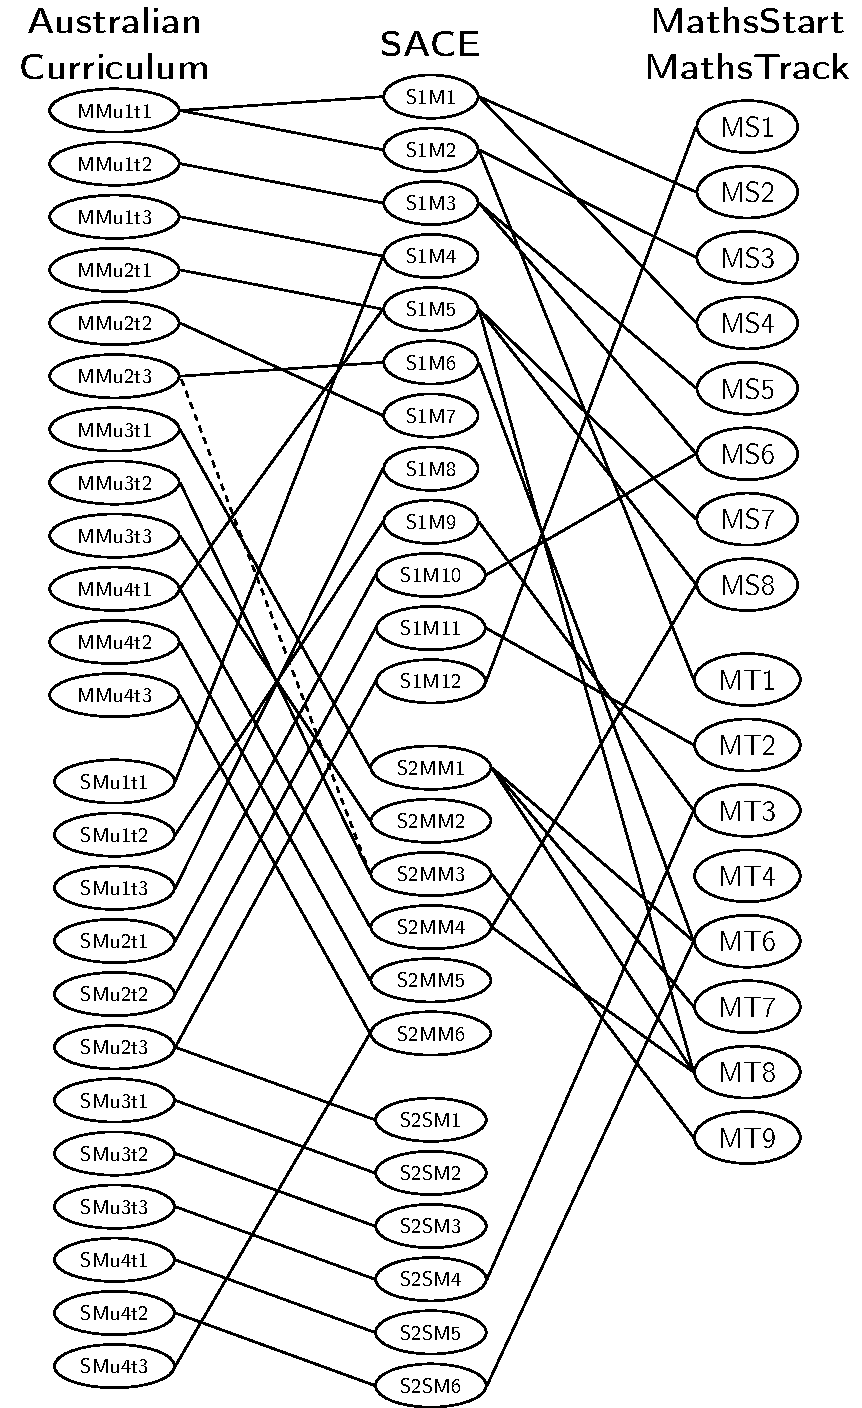
\includegraphics[scale=0.32]{../figures/mapping.pdf}
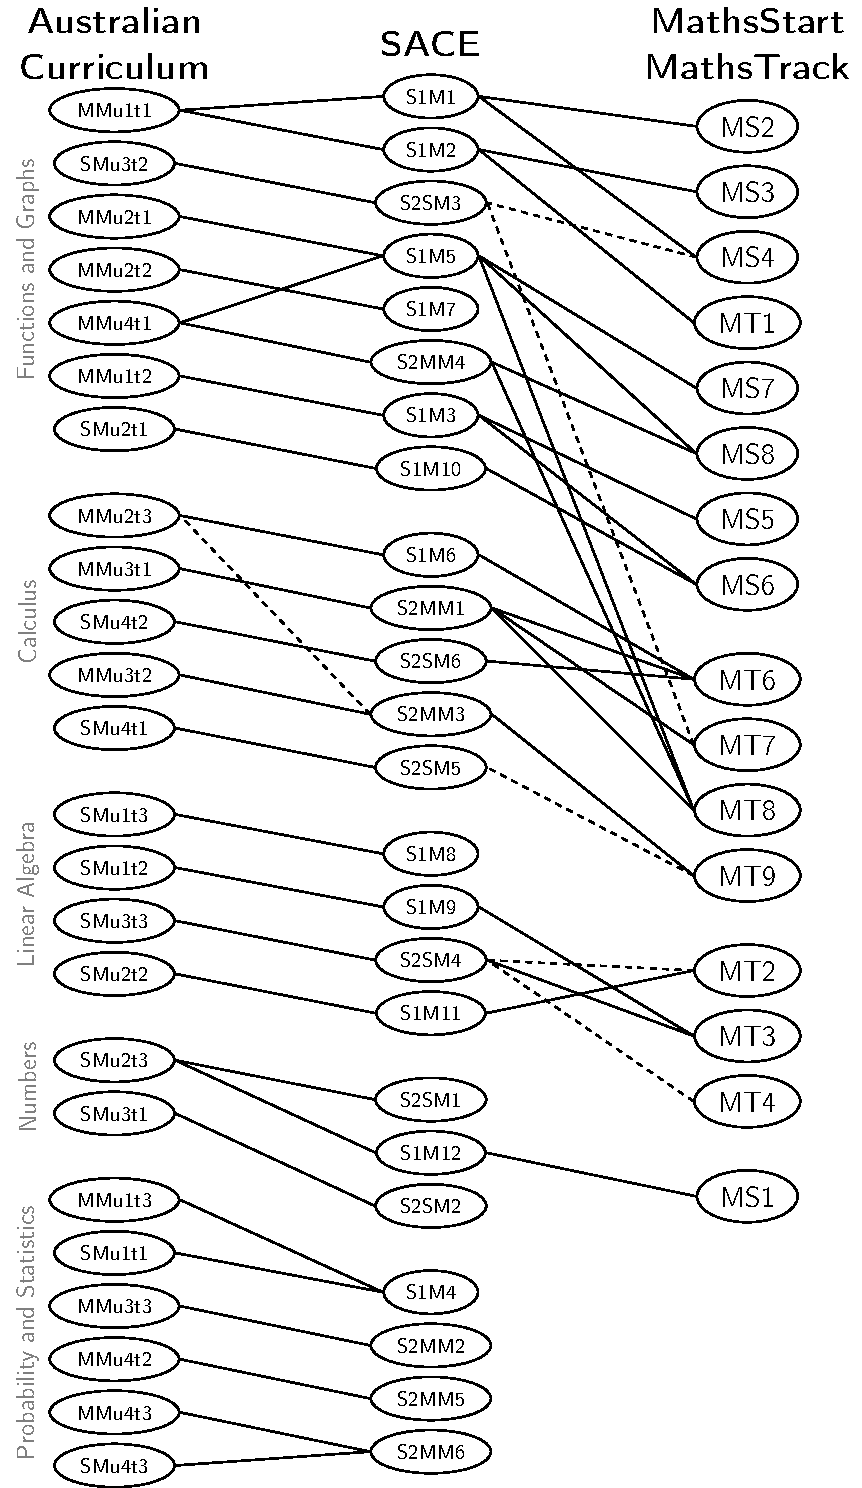
\includegraphics[scale=0.32]{../figures/mappingByTopic.pdf}
\end{center}
% Prob and Stats is where AC and SACE diverge the most, with AC taking a much more theoretical approach introducing set-theoretic notation, more combinatorics, and discussing theories explicitly. SACE on the other hand takes a much more practical approach of focussing on the calculation of statistics: mean median, mode, etc. instead, and notably skips the concept of a CDF entirely.
% My dissertation contains over 6 pages of recommendations on adjustments that could be made to the bridging courses to bring them into closer alignment with SACE/ AC.
\end{frame}

\section{Recommendations \& Conlusions}

\begin{frame}
\frametitle{Recommendations}
\begin{itemize}
	\item SET CLEAR EXPECTATIONS.
	\item Encourage Social Interaction Between Students.
	\item Adjust content to better align with the national curriculum but do so gradually, with a keen eye on students affective reactions to content as the priority.
\end{itemize}
\end{frame}

\begin{frame}
\frametitle{Impact \& Conclusions}
Bridging courses have the opportunity to:
\begin{itemize}
	\item provide students with a path towards a mathematics education, and the social mobility that entails, that they might otherwise not have had access too.
	\item have an impact on students' affect towards mathematics, and hence also
	\item help students to succeed both in mathematics education and in life.
\end{itemize}
\end{frame}

\begin{frame}
\frametitle{APST}
\begin{itemize}
	\item 1.1: Physical, social and intellectual development and characteristics of students
	\item 1.2: Understand how students learn
	\item 2.1: Content and teaching strategies of the teaching area
	\item 2.2: Content selection and organisation
	\item 2.3: Curriculum, assessment and reporting
	\item 3.6: Evaluate and improve teaching programs
	\item 4.1: Support student participation
	\item 6.3: Engage with colleagues and improve practice
\end{itemize}
% NOTE: These are just the most relevant APST, but others (in particular supporting ATSI students, students with disability, and students with english as an additional languag) are also very relevant here, simply where not an explicit focus on this work.
\end{frame}


\begin{frame}
\begin{center}
{\Huge
Questions?
}
\end{center}
\end{frame}

% Bibliography/ References
\begin{frame}[allowframebreaks]
    \frametitle{References}
	\bibliographystyle{apacite}
	\bibliography{../citations} 
\end{frame}






\end{document}


